\chapter{Tag 10 — Vom Verständnis zum Code}

\begin{quote}
Gestern hast du eine Stunde lang einen einzigen EAN-13 von Hand
gezeichnet. Heute schreibst du ein Python-Programm, das das in einer
Hundertstelsekunde macht — und für \emph{jeden} EAN-13. Der eigentliche
Stoff heute ist nicht Pillow (das Werkzeug ist klein), sondern: \emph{wie
übersetzt man ein verstandenes Encoding in Code}? Wir machen das in
drei Stufen — vom „dummen" bis zum kompakten.
\end{quote}

\section*{Lernziele für heute}

Am Ende von Tag 10 kannst du \dots

\begin{itemize}
\item die Pillow-Bibliothek in Thonny installieren und mit fünf
  Befehlen ein schwarz-weißes Bild erzeugen
\item Codetabellen aus dem Buch in Python-\emph{Dictionaries} übersetzen
  und mit eckigen Klammern darin nachschlagen
\item denselben Algorithmus in drei Versionen schreiben — explizit
  mit jeder Position einzeln, dann mit einer \texttt{for}-Schleife,
  und schließlich kompakt mit \texttt{enumerate}
\item den EAN-13 von deinem Honigglas mit Python rendern und mit
  deiner Hand-Zeichnung Modul für Modul vergleichen
\end{itemize}

\paragraph{Was du heute neu lernen wirst}
Drei Python-Bauteile, die in den Etappen vorher noch nicht
vorgekommen sind:

\begin{itemize}
\item \textbf{Dictionary} (\texttt{\{"a": 1, "b": 2\}}): eine
  Tabelle, in der man mit dem Schlüssel den Wert nachschlägt
\item \textbf{\texttt{enumerate}}: eine Schleife, die Index
  \emph{und} Wert gleichzeitig liefert
\item \textbf{Komposition kleiner Funktionen}: aus Bausteinen ein
  ganzes Programm zusammensetzen
\end{itemize}

\paragraph{Material} Laptop mit Thonny, Internetverbindung (zum
einmaligen Pillow-Installieren), die Werkstatt-Bögen aus Tag 9 zum
Vergleichen. Optional: ein Drucker, um die Python-Strichcodes neben
deine Hand-Zeichnung zu legen.

% =============================================================
\section{Pillow in Thonny einrichten \normalfont(\textit{≈ 10 min})}
% =============================================================

\textbf{Pillow} ist eine Bibliothek für Bilder — Pixel setzen,
Rechtecke zeichnen, PNGs speichern. Sie ist nicht Teil der
Standard-Python-Installation, du musst sie einmalig nachinstallieren.

\begin{werkzeugcheck}{Pillow installieren}
In Thonny: \textbf{Tools → Manage Packages\dots} öffnen. Im Suchfeld
\texttt{Pillow} eintippen, das gefundene Paket markieren,
\textbf{Install} drücken. Lade etwa 4 MB; nach ein paar Sekunden
erscheint \texttt{Pillow} unten in der Liste der installierten Pakete.

Lass dir helfen, falls die Installation nicht klappt — Firewalls und
Schul-Netzwerke machen manchmal Probleme.
\end{werkzeugcheck}

\begin{pythoneinheit}{1}{Smoke-Test}
\pythoncodeteil{tag10/pillow_basics.py}{installprobe}

Wenn das Programm \texttt{PIL.Image läuft.} ausgibt, ist alles in
Ordnung. Bei \texttt{ModuleNotFoundError: No module named 'PIL'} hat
die Installation nicht funktioniert.

\paragraph{Warum heißt es \texttt{PIL}?}
Pillow ist der Nachfolger der älteren \emph{Python Imaging Library}
(„PIL"); der Modul-Name aus dem Original wurde beibehalten. Beim
Importieren schreibt man also \texttt{from PIL import Image}, obwohl
das Paket heute \texttt{Pillow} heißt.
\end{pythoneinheit}

\begin{pythoneinheit}{2}{Ein erster Strich}
\pythoncodeteil{tag10/pillow_basics.py}{erstes_bild}

Drei Zeilen Pillow-Pflicht — mehr brauchst du heute nicht zu kennen:

\begin{enumerate}
\item \texttt{Image.new("1", (breite, höhe), 1)} erzeugt ein Bild
  im Modus „1" (= ein Bit pro Pixel, schwarz oder weiß), mit
  weißem Hintergrund (\texttt{1}).
\item \texttt{ImageDraw.Draw(bild)} liefert ein Zeichen-Objekt,
  das in das Bild reinmalt.
\item \texttt{rectangle([(x0,y0),(x1,y1)], fill=0)} zeichnet
  ein schwarzes Rechteck.
\item \texttt{bild.save("name.png")} speichert das Ergebnis.
\end{enumerate}

Das Resultat:

\begin{center}
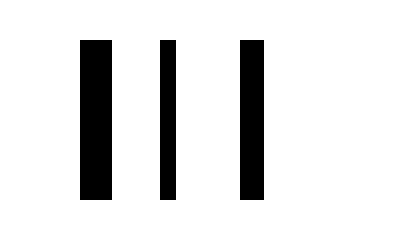
\includegraphics[width=4cm]{abbildungen/tag10/drei_striche_zoom.png}
\end{center}

(genauer: ein einzelner Strich, hier auf 8-fache Größe vergrößert
damit man die Pixel sieht — wir nehmen das Bild aus Etappe 9 als
Anker für „Modul für Modul"-Denken.)
\end{pythoneinheit}

% =============================================================
\section{Tabellen werden zu Dictionaries \normalfont(\textit{≈ 15 min})}
% =============================================================

In Etappe 9 hattest du auf dem Werkstatt-Spickzettel eine Tabelle: pro
Ziffer 0 bis 9 stand der L-Code, der G-Code, der R-Code. Mit dem
Finger hast du die Zeile zur Ziffer gesucht und das passende 7-Bit-
Muster abgelesen.

In Python heißt diese Datenstruktur \textbf{Dictionary}.

\paragraph{Was ist ein Dictionary?}
Ein Dictionary (kurz: \emph{Dict}) ist eine Tabelle in Code-Form. Man
schreibt sie mit geschweiften Klammern; jeder Eintrag besteht aus
einem \emph{Schlüssel} und einem \emph{Wert}, getrennt durch einen
Doppelpunkt. Beispiel:

\begin{minted}{python}
farben = {"apfel": "rot", "banane": "gelb", "kiwi": "grün"}
\end{minted}

Hier sind \texttt{"apfel"}, \texttt{"banane"} und \texttt{"kiwi"} die
Schlüssel; \texttt{"rot"}, \texttt{"gelb"} und \texttt{"grün"} die
Werte. Jetzt kannst du nachschlagen — wie in einem Wörterbuch:

\begin{minted}{python}
>>> farben["banane"]
'gelb'
>>> farben["apfel"]
'rot'
\end{minted}

Mit \emph{eckigen} Klammern und dem Schlüssel bekommst du den Wert.
Du kennst diese Schreibweise schon von \emph{Listen} (\texttt{liste[0]}
ist das erste Element); bei Dictionaries ist statt einer Zahl ein
Schlüssel deiner Wahl drin.

\paragraph{Warum nicht einfach eine Liste?}
Mit einer Liste müsstest du dir merken: „die Banane ist Element Nummer 1".
Bei einem Dict steht direkt \texttt{farben["banane"]} — selbsterklärend
und unabhängig von der Reihenfolge. Genau das, was wir für unsere
Codetabellen brauchen: \texttt{L\_CODES["2"]} ist eindeutig der L-Code
für die Ziffer 2 — egal, wo der im Dict steht.

\begin{bleistiftuebung}{1}{Pattern entschlüsseln}
Unser Honig-EAN ist \texttt{4270004371635}. Aus der Pattern-Tabelle
weißt du: bei Erstziffer \texttt{4} ist das Pattern \texttt{LGLLGG}.

Schreibe eine kleine Tabelle auf Papier: für jede der sechs linken
Datenziffern (Position 2 bis 7) die Ziffer selbst, das passende
Pattern-Zeichen (L oder G), und den Code, den du im Spickzettel
nachschlagen würdest. Beispielzeile:

\begin{center}
\small
\begin{tabular}{c c c c}
\toprule
Position & Ziffer & Pattern & Code \\
\midrule
2 & 2 & L & \texttt{0010011} \\
3 & ? & ? & ? \\
\dots \\
\bottomrule
\end{tabular}
\end{center}

Das ist \emph{exakt} der Algorithmus, den wir gleich in Python
schreiben — du machst ihn jetzt einmal von Hand, damit dir der
Code nichts Magisches mehr ist.
\end{bleistiftuebung}

\begin{pythoneinheit}{3}{Codetabellen als Dictionaries}
\pythoncodeteil{tag10/ean13_encoder.py}{tabellen}

Vier Dictionaries: drei für die Codetabellen, eine für die Pattern.
Du tippst sie einmal ab — danach hast du das ganze Encoding-Wissen
aus Etappe 9 in einer Datei.

\paragraph{Probier in Thonnys interaktiver Konsole}

\begin{minted}{python}
>>> L_CODES["2"]
'0010011'
>>> PATTERNS["4"]
'LGLLGG'
>>> PATTERNS["4"][0]
'L'
\end{minted}

Mit \texttt{PATTERNS["4"]} bekommst du den ganzen Pattern-String,
mit \texttt{PATTERNS["4"][0]} das erste Zeichen davon. Strings
verhalten sich also auch ein bisschen wie Dictionaries — man kann
mit eckigen Klammern und Index drin nachschlagen.
\end{pythoneinheit}

% =============================================================
\section{Stufe 1 — alles ausgeschrieben \normalfont(\textit{≈ 15 min})}
% =============================================================

Bevor wir Schleifen einsetzen, schreiben wir den Algorithmus einmal
\emph{komplett ausgeschrieben} hin. Das wird lang und repetitiv —
genau das ist der Punkt: jeder Schritt steht klar da, du siehst, was
passiert. Schleifen sind dann „diese sechs Zeilen, aber kompakter".

\begin{pythoneinheit}{4}{Linke Hälfte ohne Schleife}
\pythoncodeteil{tag10/ean13_encoder.py}{stufe1_dumm}

\paragraph{Was hier passiert (Zeile für Zeile)}
\begin{enumerate}
\item \texttt{ean[0]} ist die Erstziffer \texttt{"4"}; \texttt{PATTERNS[ean[0]]}
  schlägt das Pattern \texttt{"LGLLGG"} nach.
\item \texttt{bits = "101"} startet mit dem Start-Guard.
\item Für Position 2 (\texttt{ean[1]} ist \texttt{"2"}) ist
  \texttt{pattern[0]} ein \texttt{"L"} — also nimmt der Code
  \texttt{L\_CODES[ean[1]]} und hängt das an \texttt{bits} an.
\item Für Position 3 ist \texttt{pattern[1]} ein \texttt{"G"} — also
  \texttt{G\_CODES[ean[2]]}. Und so weiter, sechs Mal nach demselben
  Schema.
\item Am Ende kommt der Mittel-Guard.
\end{enumerate}

Wenn du das Skript laufen lässt, druckt es die Anzahl der Bits, die
zusammengekommen sind — sollten 50 sein
(3 + 6$\times$7 + 5 = 50, denn die rechte Hälfte und der End-Guard
fehlen noch). Probier's.
\end{pythoneinheit}

% =============================================================
\section{Stufe 2 — eine Schleife statt sechs Wiederholungen \normalfont(\textit{≈ 15 min})}
% =============================================================

Sechs identisch gebaute \texttt{if}-Blöcke nacheinander — das ist
genau der Moment, wo eine Schleife angebracht ist. Wir schreiben den
gleichen Algorithmus mit einer einzigen \texttt{for}-Schleife.

\begin{pythoneinheit}{5}{Mit Schleife}
\pythoncodeteil{tag10/ean13_encoder.py}{stufe2_loop}

Was sich gegenüber Stufe 1 geändert hat: statt sechs Mal denselben
Code mit unterschiedlichen Indizes zu schreiben, lassen wir die
Schleifen-Variable \texttt{i} von 0 bis 5 laufen. Innen drin steht
einmal die Logik — \texttt{pattern[i]} ist das jeweils richtige
Pattern-Zeichen, \texttt{ean[i+1]} die jeweils richtige EAN-Ziffer.

\paragraph{Warum \texttt{ean[i+1]} und nicht \texttt{ean[i]}?}
Position 2 im EAN ist Index 1 (Index 0 wäre die Erstziffer, die wir
ja nicht zeichnen). Bei \texttt{i = 0} wollen wir also Position 2,
das ist \texttt{ean[1]} — daher der Versatz \texttt{+1}.

Jetzt sind es \emph{volle 95 Bits} — die zweite Schleife für die
rechte Hälfte funktioniert genauso, nur mit \texttt{R\_CODES} (kein
Pattern, weil rechts alles R-codiert ist).
\end{pythoneinheit}

\begin{bleistiftuebung}{2}{Stufe 1 vs. Stufe 2 vergleichen}
Halte beide Code-Versionen nebeneinander. Was ist \emph{semantisch}
gleich (was tut der Code), und was ist \emph{syntaktisch} anders (wie
ist er geschrieben)? Welche Version würdest du Greta in einem Jahr
zeigen, wenn sie EAN-13 schon vergessen hat? Welche, wenn sie zum
ersten Mal hinguckt?
\end{bleistiftuebung}

% =============================================================
\section{Stufe 3 — \texttt{enumerate} liefert Index \emph{und} Wert \normalfont(\textit{≈ 15 min})}
% =============================================================

In Stufe 2 mussten wir bei jedem Schleifendurchlauf \texttt{ean[i+1]}
schreiben, um an die Ziffer zu kommen. Python hat dafür ein hübsches
Hilfsmittel: \texttt{enumerate(...)} läuft über eine Liste und liefert
\emph{Index und Wert in einem}.

\paragraph{enumerate — Index und Wert gleichzeitig}
Du hast \texttt{enumerate} schon in Tag 1 beim EAN-13-Validator
benutzt — falls dir das nicht mehr präsent ist, hier die Kurzform:

\begin{minted}{python}
>>> for i, ch in enumerate("LGLLGG"):
...     print(i, ch)
0 L
1 G
2 L
3 L
4 G
5 G
\end{minted}

Statt nur über die Werte zu laufen (\texttt{for ch in "LGLLGG":}),
liefert \texttt{enumerate} \emph{zwei} Variablen pro Durchlauf: einen
laufenden Index (hier \texttt{i}) und den jeweiligen Wert (hier
\texttt{ch}). Praktisch, wenn du \emph{beides} brauchst — wie bei
unserem Encoder.

\paragraph{Slicing — ein Stück aus einem String herausnehmen}
\texttt{ean[1:7]} ist eine \emph{Slice}: nimm aus dem String
\texttt{ean} die Zeichen von Index 1 bis (\emph{ausschließlich})
Index 7 — also genau die Zeichen an Positionen 1, 2, 3, 4, 5, 6.
Beim Honig-EAN \texttt{"4270004371635"} ist das die Folge
\texttt{"270004"}.

\paragraph{Die Kurzform \texttt{bits += \dots}}
\texttt{bits += L\_CODES[ziffer]} ist die Kurzform für
\texttt{bits = bits + L\_CODES[ziffer]}. Spart Tipperei und ist
weniger fehleranfällig; in Python sehr üblich.

\begin{pythoneinheit}{6}{Mit enumerate}
\pythoncodeteil{tag10/ean13_encoder.py}{stufe3_enumerate}

Im Encoder-Code heißt die Wertvariable \texttt{ziffer} statt
\texttt{ch} — gleiche Idee. Die linke Schleife läuft über
\texttt{ean[1:7]} (die sechs linken Datenziffern), die rechte
über \texttt{ean[7:13]} (die sechs rechten).

\paragraph{Stufe 1 → 2 → 3}
Alle drei Versionen machen \emph{exakt dasselbe}. Stufe 1 ist
hilfreich zum Verstehen, Stufe 3 zum Lesen, wenn man Python kennt.
Stufe 2 ist ein guter Mittelweg, falls dir \texttt{enumerate} noch
fremd ist.
\end{pythoneinheit}

% =============================================================
\section{Aus dem Code wird eine Funktion \normalfont(\textit{≈ 10 min})}
% =============================================================

Bisher steht der Code direkt im Skript — das funktioniert, aber lässt
sich nicht wiederverwenden. Wir packen ihn in eine \emph{Funktion},
die einen EAN bekommt und die Bit-Folge zurückgibt.

\begin{pythoneinheit}{7}{Encoder als Funktion}
\pythoncodeteil{tag10/ean13_encoder.py}{funktion}

Funktion definieren mit \texttt{def}, Eingabe als Parameter
(\texttt{ean}), Ausgabe mit \texttt{return}. Aufruf:
\texttt{bits\_for\_ean("4270004371635")} gibt die 95-Bit-Folge zurück.

Test in Thonnys Konsole:

\begin{minted}{python}
>>> bits = bits_for_ean("4270004371635")
>>> len(bits)
95
>>> bits[:20]
'10100100110010001000'
\end{minted}
\end{pythoneinheit}

% =============================================================
\section{Vom Bit zum Bild \normalfont(\textit{≈ 25 min})}
% =============================================================

Jetzt fehlt nur noch der Schritt vom 95-Bit-String zum gerenderten
PNG. Pillow stellt uns Rechtecke zur Verfügung — pro \texttt{1}-Bit
malen wir ein modulbreites Rechteck.

\begin{bleistiftuebung}{3}{Geometrie planen}
Bevor du den Drawer-Code anschaust, plane auf Papier:

\begin{itemize}
\item Wenn ein Modul $4$ Pixel breit gerendert werden soll, wie breit
  ist dann ein einzelnes Datenmodul (in Pixeln)?
\item Wie breit ist die Hellzone links? (11 Module)
\item Wie viele Pixel braucht das gesamte Bild für einen EAN-13 mit
  $4$ Pixel pro Modul, einschließlich beider Hellzonen?
\end{itemize}

(Lösung: $11 + 95 + 7 = 113$ Module; bei $4$ Pixeln pro Modul also
$452$ Pixel breit.)
\end{bleistiftuebung}

\begin{pythoneinheit}{8}{Strichcode rendern}
\pythoncodeteil{tag10/ean13_encoder.py}{drawer}

\paragraph{Was hier passiert}
\begin{itemize}
\item Berechne die Bildbreite aus Modulbreite + Anzahl Module.
\item Erzeuge ein leeres weißes Bild der berechneten Größe.
\item Geh die Bit-Folge durch (\texttt{enumerate} kennst du schon).
  Pro \texttt{"1"} ein schwarzes Rechteck zeichnen, von oberem Rand
  bis unterem Rand, an Position \texttt{x0} bis \texttt{x1}.
\item Speichern.
\end{itemize}

Beachte den Offset \texttt{hellzone\_links}: das schwarze Rechteck
beginnt nicht bei x=0, sondern um die Hellzone versetzt.
\end{pythoneinheit}

\begin{pythoneinheit}{9}{Demo}
\pythoncodeteil{tag10/ean13_encoder.py}{demo}

Das ist der Honig-Code, frisch von Pillow erzeugt:

\begin{center}

\includegraphics[width=8cm]{abbildungen/tag10/honig.png}
\end{center}

Zum Vergleich: die Schokolade aus Tag 1:

\begin{center}

\includegraphics[width=8cm]{abbildungen/tag10/schokolade.png}
\end{center}

Und eine ISBN-13 (auch ein EAN-13, mit Buch-Präfix \texttt{978}):

\begin{center}

\includegraphics[width=8cm]{abbildungen/tag10/buch.png}
\end{center}
\end{pythoneinheit}

% =============================================================
\section{Diagnose — Hand vs. Python \normalfont(\textit{≈ 10 min})}
% =============================================================

\begin{bleistiftuebung}{4}{Modul-für-Modul-Vergleich}
Drucke deinen Python-Honig-Code aus (oder lies ihn am Bildschirm
ab) und lege ihn neben deine Hand-Zeichnung von gestern. Geh Modul
für Modul von links nach rechts: ist jeder schwarze Strich an
derselben Position? Findest du eine Stelle, an der dein Hand-Code
\emph{nicht} mit dem Python-Code übereinstimmt?

Wenn ja: war es ein Fehler in der Hand-Zeichnung — oder im Python-
Code? Wie könntest du das herausfinden?
\end{bleistiftuebung}

% =============================================================
\section{Reflexion und Brücke zu Datamatrix \normalfont(\textit{≈ 10 min})}
% =============================================================

Du hast jetzt zwei Wege, einen EAN-13 herzustellen — beide brauchen
\emph{exakt dasselbe Wissen} aus Etappe 9. Python nimmt dir das
Verstehen nicht ab, sondern nur das Tun. Was beim Hand-Zeichnen eine
Stunde dauert, ist mit Python eine Hundertstelsekunde. Skalierung ist
das Argument.

Ebenso wichtig wie der Encoder selbst sind die drei Stufen — sie
zeigen, wie Code „dichter" wird, je mehr Sprachmittel du beherrschst.
Stufe 1 ist nicht falsch, nur lang. Stufe 3 ist nicht magisch, nur
kompakt. Wenn du eine Sprache neu lernst, ist Stufe 1 oft der
Startpunkt und Stufe 3 das Ziel — aber keiner schreibt von Anfang
an Stufe 3.

\paragraph{Was geht damit?}
Du kannst Strichcodes auf Vorrat erzeugen. Eine Etiketten-Vorlage,
ein Drucker, ein Skript — und du klebst eigene EANs auf alles, was
du katalogisieren willst. Oder ein Familien-Quiz: jeder bekommt
seinen Geburtsdatum-EAN als Code-Karte.

\paragraph{Was geht (noch) nicht?}
Der \emph{Decoder} — also ein Programm, das ein PNG einliest und
die 13 Ziffern zurückgibt. Das ist deutlich kniffliger als der
Encoder (Pixel-Toleranz, Bildverzerrung, Helligkeit), kein Pflicht-
Stoff für unsere zwei Wochen. Bei Interesse als Bonus-Aufgabe.

\subsection*{Vorschau Tag 11 — Datamatrix-Symbol}

EAN-13 ist ein 1D-Strichcode: alles in einer Zeile. Datamatrix ist
2D — schwarze und weiße Module in einem quadratischen Raster, wie
ein Mini-Schachbrett mit Bedeutung. Was heute drei Datentypen waren
(L, G, R), werden bei Datamatrix \emph{Hunderte} Module — und
mittendrin: die Reed-Solomon-Prüfsymbole, die wir an den Tagen 6 bis
8 berechnet haben. Datamatrix kann \emph{Fehler korrigieren}:
gestempelte Symbole auf Versandetiketten überstehen Knicke, Wasser
und Filzstift.
